% !Mode:: "TeX:UTF-8"
\documentclass{../common/tufte-latex/tufte-handout}

\title{Git hands-on, part I-b: Appendix}

\author{S\'ebastien Dawans}

\date{07 February 2014} % without \date command, current date is supplied

%\geometry{showframe} % display margins for debugging page layout
\usepackage[utf8]{inputenc}
\usepackage{graphicx} % allow embedded images
  \setkeys{Gin}{width=\linewidth,totalheight=\textheight,keepaspectratio}
  \graphicspath{{graphics/}} % set of paths to search for images
\usepackage{amsmath}  % extended mathematics
\usepackage{booktabs} % book-quality tables
\usepackage{units}    % non-stacked fractions and better unit spacing
\usepackage{multicol} % multiple column layout facilities
\usepackage{lipsum}   % filler text
\usepackage{fancyvrb} % extended verbatim environments
  \fvset{fontsize=\normalsize}% default font size for fancy-verbatim environments
\usepackage{listings}
\lstset{showstringspaces=false}
\usepackage[usenames]{xcolor}

\lstdefinestyle{BashInputStyle}{
  language=bash,
  basicstyle=\footnotesize\ttfamily,
  %numbers=left,
  %numberstyle=\tiny,
  %numbersep=3pt,
  frame=tb,
  columns=fullflexible,
  backgroundcolor=\color{yellow!20},
  linewidth=0.95\linewidth,
  xleftmargin=0.05\linewidth,
  moredelim=**[is][\color{red}]{§}{§},
  moredelim=**[is][\color{OliveGreen}]{`}{`}
}

% Standardize command font styles and environments
\newcommand{\doccmd}[1]{\texttt{\textbackslash#1}}% command name -- adds backslash automatically
\newcommand{\docopt}[1]{\ensuremath{\langle}\textrm{\textit{#1}}\ensuremath{\rangle}}% optional command argument
\newcommand{\docarg}[1]{\textrm{\textit{#1}}}% (required) command argument
\newcommand{\docenv}[1]{\textsf{#1}}% environment name
\newcommand{\docpkg}[1]{\texttt{#1}}% package name
\newcommand{\doccls}[1]{\texttt{#1}}% document class name
\newcommand{\docclsopt}[1]{\texttt{#1}}% document class option name
\newenvironment{docspec}{\begin{quote}\noindent}{\end{quote}}% command specification environment

\begin{document}

\maketitle% this prints the handout title, author, and date

\begin{abstract}
\noindent
This handout complements the information given in the previous handout, \textbf{part I: single user operations}.
The first part looks at how to ignore files from Git.
The rest documents the history modification commands that were introduced orally during the last session in answer to specific questions.
\end{abstract}

\section{Ignoring files}
In many source code directories, there are files which we do not want to (or should not) version control.
Any file which is generated from source code and likely to change at every compilation of the project should not be version controlled.
Likewise, huge files should be handled by other means, even if these are not necessarily regenerated and are a required dependency for a project compilation or runtime like a library.
To handle this, Git can be told to ignore certain files by pattern rules.
Ignored untracked files will stay untracked without polluting the \textbf{git status} output.

\subsection{Using .gitignore files}
There are several ways of instructing git to ignore files by pattern rules, the most common one is by means of \textbf{.gitignore} files placed in the working tree and version-controlled in the same way as a normal file.
\marginnote{Type \textbf{git help gitignore} for a list of other ways to ignore files. Note that there is an order of precedence.}

It is important to define a \textbf{.gitignore} file as early on in a Git project as possible.
When creating a new project from scratch, it's good practice to include a .gitignore file in the first commit, even if empty.
When adding an existing code base to Git, it's even more important to get the .gitignore right before adding the whole project recursively, because there might already exist some files which you need to ignore.

\noindent \textbf{Example}.
Consider a very simple C project with .c files, a Makefile and a generated binary.
Suppose we have just created a \texttt{hello.c} file, adapted our Makefile and compiled it:

\begin{lstlisting}[style=BashInputStyle]
  $ git status
  On branch master
  Untracked files:
    (use "git add <file>..." to include in what will be committed)
  
      §Makefile§
      §hello.c§
      §hello.exe§

nothing added to commit but untracked files present (use "git add" to track)
\end{lstlisting}

If we type \texttt{git add .} at this point, all three files will be added to Git.
Suppose we wanted to ignore the generated file, we could decide to exlude all files ending in ".exe", let's create a file called .gitignore and add \textbf{*.exe} on the first line:
\begin{lstlisting}[style=BashInputStyle]
  $ touch .gitignore
  $ echo "*.exe" >> .gitignore
\end{lstlisting}

The next time we look at \texttt{git status}, it will be ignored:
\begin{lstlisting}[style=BashInputStyle]
  $ git status
  On branch master
  Untracked files:
    (use "git add <file>..." to include in what will be committed)
  
      §.gitignore§
      §Makefile§
      §hello.c§

nothing added to commit but untracked files present (use "git add" to track)
\end{lstlisting}

Notice that we have a new untracked file, our new .gitignore file.
We can now add the whole project and make our first commit.

\begin{lstlisting}[style=BashInputStyle]
  $ git add .
  $ git commit -m "Initial Commit: adding the project files"
\end{lstlisting}

In Git the .gitignore files are part of the working tree and must be committed like any other source file.
This is very convenient because it allows to propagate the rules of ignored files.
Regular users of a project thus do not usually worry about .gitignores, the work of defining ignored files having already been done by the project owner, who knows best which files should be ignored.

\subsection{Forgot to ignore some files?}
At some point you might forget to include a certain pattern in a .gitignore.
If some files have accidentally been added to version control when they should not have, it is easy to ignore them later.
Assuming that the file is not required to be on the repository, we have already learned the required command in the previous lesson: \texttt{git rm} with the \texttt{cached} option.

Suppose we have a \texttt{hello.exe} binary file part of the repository which we want to untrack and ignore, we would do:
\marginnote{The \textbf{cached} option preserves a local copy of hello.exe, which isn't really necessary since we know we can just regenerate it with our Makefile}
\begin{lstlisting}[style=BashInputStyle]
  $ git rm --cached hello.exe
  $ echo "*.exe" >> .gitignore
  $ git add .gitignore
  $ git commit -m "Remove file hello.exe and ignore all *.exe files"
\end{lstlisting}

Note that this procedure is \textbf{not sufficient if you are concerned with removing a huge binary file from a git repository} for performance reasons, because it is still contained in the history and the blob in the git objects database is still there.
Permanently removing the objects from the repository requires all the refs on the blob to be removed, followed by a garbage collection of the unreferences blobs.
This is not trivial and definately out of scope of our lesson.

\subsection{Ignoring a versioned file without removing it from Git}
In some projects, it is sometimes necessary to ignore local modifications of a certain file but not remove the file from version control.
An example of this is when a developer needs to change parts of a file to match a certain local setting, like activating a debugging flag in a file or specifiying credentials like database login/password in a script interacting with a database.
Ignoring modifications to such files cleans your git status and also avoid you to accidentally commit those changes if you use shortcuts like \texttt{git commit -a}.
You cannot simply use a local (untracked) .gitignore file for this, because \textbf{.gitignore only applies to untracked files}; you cannot ignore a file already part of the repository.
\marginnote{A local, uncommitted .gitignore file would not be a clean way even if it was possible, because the .gitignore file itself would appear as untracked every time you type git status.}

Although git stash does the trick, git stash will actually hide your modifications from the working tree so you would need to stash and unstash your local modifications everytime you want to commit.

An simpler alternative is to temporarily ignore local changes in a file:
\begin{lstlisting}[style=BashInputStyle]
  $ git update-index --assume-unchanged <file>
\end{lstlisting}

This activates a certain flag on the file and marks it as ignored by Git.
The file will still receive updates from upstream, but local modifications will be ignored.
To undo this:

\begin{lstlisting}[style=BashInputStyle]
  $ git update-index --no-assume-unchanged <file>
\end{lstlisting}

You can obtain a list of all files ignore in this way using:

\begin{lstlisting}[style=BashInputStyle]
  $ git ls-files -v | grep ^[a-z]
\end{lstlisting}

The following 3 aliases are useful to add in your ~/.gitconfig:

\begin{lstlisting}[style=BashInputStyle]
[alias]
        ignore = !git update-index --assume-unchanged 
        unignore = !git update-index --no-assume-unchanged
        ignored = !git ls-files -v | grep ^[a-z]
\end{lstlisting}

\section{Rewriting History}
Git gives lots of power to the user and allows to rewrite the history.
This can be \textbf{rewording} commit messages, \textbf{combining} commits, \textbf{splitting} a large commit into smaller ones, \textbf{deleting} a commit, \textbf{reordering} commits, changing the \textbf{date and authoring} information, etc.

\noindent \textbf{Warning}. Changing the history of a branch which has already been shared to other people is not a good practice, because those people will have to hard reset their work to your new branch and apply their modifications on top of it.
\marginnote{Rewriting history is a great way of cleaning one's work before pushing, but should not be used a posteriori on an important branch (master, develop).}
If you ever have doubts about when it is ok or not to rewrite history, use this simple \textbf{rule: do not modify history pushed on a shared repository}.

\subsection{Amending the last commit}
The simplest form of history modification is changing the last commit:

\begin{lstlisting}[style=BashInputStyle]
  $ git commit --amend
\end{lstlisting}

This command opens up the last commit message, and allows you to alter the message.
It then takes whatever is in the staging area and adds it to the previous commit, with the new commit message, instead of creating a new commit.
Thus, this is for both \textbf{rewording the last commit} and \textbf{appending more changes to the last commit}.

Let's reword the last commit message of lesson1 in its initial state:

\begin{lstlisting}[style=BashInputStyle]
  $ git clone git@gitlab.server.com:login/lesson1
  $ cd lesson1
  $ git log --oneline
  $ gitk --all
  $ git commit --amend -m "New message"
  $ git log --oneline
  $ gitk --all
\end{lstlisting}

\begin{figure*}%
  \centering
  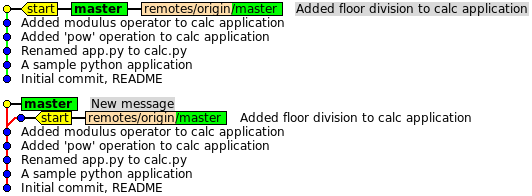
\includegraphics[width=0.85\linewidth]{gitcommit-amend.png}
  \label{fig:gitcommit-amend}
  \caption{Before (top) and after (bottom) amending the last commit message}
\end{figure*}

The output of gitk at the 2 steps is shown in Figure \ref{fig:gitcommit-amend}.
We can see that ammending the commit creates a divergence between out local master branch's history and that of the remote's.
The change in history means \textbf{you cannot git push}. 
In fact, doing so will raise an error because git refuses to push work on a branch which does not pick up from the branch's last commit in its exact state (hash value).

\subsection{More thorough history modifications with interactive rebase}
Amending the last commit only scratches the surface of history modifications.
A more general and powerful command to edit history is the interactive rebase command.

To \textbf{rebase} the HEAD on a certain tree-ish, means to:

\begin{enumerate} 
 \item{rewind both the HEAD and the specified tree-ish until obtaining a common point in history}
 \item{apply the commits belonging to HEAD, missing from the tree-ish on top of that tree-ish}
 \item{continuously move the current HEAD to the latest commit as the patches are applied}
\end{enumerate}

This is a very general command used in different contexts.
When applying each commit on the new base, we can tell git to perform extra operations are each step when invoking \textbf{rebase in interactive mode}.
This is particularly convenient for rewriting history: we simply rebase the current HEAD on a commit in the direct history.

Suppose we wanted to alter the commit messages of HEAD\textasciitilde1 and HEAD\textasciitilde2, we would do:
\marginnote{Reminder: HEAD\textasciitilde n is a shortcut to designate the n+1 th last commit (i.e. n commits behind the latest commit)}
\begin{lstlisting}[style=BashInputStyle]
  $ git rebase -i HEAD~3
\end{lstlisting}

The means we take the HEAD, and rebase it on a commit which is 3 commits away.
This will undo HEAD, HEAD\textasciitilde1 and HEAD\textasciitilde2, and apply them on top of HEAD\textasciitilde3 in reverse order (HEAD\textasciitilde2, HEAD\textasciitilde1, HEAD).
With the -i option, an editor pops up to prompt us if we want to take any action when picking each commit:

\begin{lstlisting}[style=BashInputStyle]
  pick 21471dd Added 'pow' operation to calc application
  pick 511d31d Added modulus operator to calc application
  pick 87854e9 New message
\end{lstlisting}

We will ask to edit 2 of the commits by replacing the 'pick' header of the appropriate lines:

\begin{lstlisting}[style=BashInputStyle]
  edit 21471dd Added 'pow' operation to calc application
  edit 511d31d Added modulus operator to calc application
  pick 87854e9 New message
\end{lstlisting}

When closing the editor, git will take each commit from top to bottom and perform the requested action.
The first action is to pick and edit 21471dd, so git will stop immediately to allow the user to amend the commit:

\begin{lstlisting}[style=BashInputStyle]
Stopped at 21471dd... Added 'pow' operation to calc application
You can amend the commit now, with

	git commit --amend

Once you are satisfied with your changes, run

	git rebase --continue
\end{lstlisting}

Let's follow Git's suggestions and amend the commit and continue the rebase operation:

\begin{lstlisting}[style=BashInputStyle]
git commit --amend -m "New commit message 1"
git rebase --continue
\end{lstlisting}

We get a similar message as before saying Git has stopped on commit 511d31d.
Again, we amend and continue the rebase:

\begin{lstlisting}[style=BashInputStyle]
git commit --amend -m "New commit message 2"
git rebase --continue
\end{lstlisting}

Git will automatically end the rebase operation when there are not more inputs required.
Our last commit is in 'pick' mode, so it is automatically picked without a user prompt.
The final history after the first amend operation and this rebase and its relationship to the remote master branch is shown in Figure \ref{fig:gitrebase-amend}.

\begin{figure*}%
  \centering
  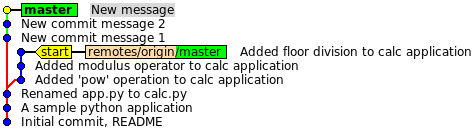
\includegraphics[width=0.75\linewidth]{gitrebase-amend.png}
  \label{fig:gitrebase-amend}
  \caption{Result of amending the last 3 commit messages}
\end{figure*}

\noindent We have covered the general mechanism of git rebase in interactive mode. 
We will now have a small preview of more advances operation which can be done with rebase.
First, let's undo out changes by reset or local master branch to the state of origin/master:

\begin{lstlisting}[style=BashInputStyle]
  git reset --hard origin/master
\end{lstlisting}

\noindent \textbf{Squashing Commits}.
A number of small commits can be combined into one.

This is done using the \textbf{squash} keyword in the git rebase editor.
Let's combine HEAD~1 and HEAD~2:

\begin{lstlisting}[style=BashInputStyle]
  $ git rebase -i HEAD~3
\end{lstlisting}

This time, we modify the rebase editor like the following:
\marginnote{The \textbf{squash} action combines a commit with the previous one, so we need to add squash to the \textbf{lower} element of a pair of commits}
\begin{lstlisting}[style=BashInputStyle]
  pick 21471dd Added 'pow' operation to calc application
  squash 511d31d Added modulus operator to calc application
  pick 87854e9 New message
\end{lstlisting}

When rebasing this, Git first picks 21471dd, then amends it with 511d31d.
An editor opens promoting for the new commit message of the combined commit:
\marginnote{In fact, the squashing in Git is pretty smart: if you squash more than 2 consecutive commits, they will all appear together in this step.}
\begin{lstlisting}[style=BashInputStyle]
# This is a combination of 2 commits.
# The first commit's message is:

Added 'pow' operation to calc application

# This is the 2nd commit message:

Added modulus operator to calc application
\end{lstlisting}

Let's modify it to:

\begin{lstlisting}[style=BashInputStyle]
Added 'pow' and 'modulus' operators
\end{lstlisting}

\begin{lstlisting}[style=BashInputStyle]
  $ git rebase --continue
\end{lstlisting}

The rebase will complete and our new history is shown in Figure \ref{fig:gitrebase-squash}

\begin{figure*}%
  \centering
  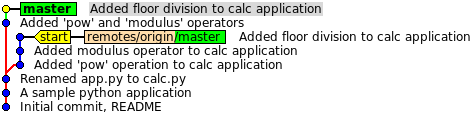
\includegraphics[width=0.75\linewidth]{gitrebase-squash.png}
  \label{fig:gitrebase-squash}
  \caption{Result of a squash in a git rebase}
\end{figure*}

Let's reset our branch again before the next part:

\begin{lstlisting}[style=BashInputStyle]
  git reset --hard origin/master
\end{lstlisting}

\noindent \textbf{Splitting a commit into smaller commits}
Splitting a large commit into smaller ones is also possible, but slightly trickier.
The keyword to use in the interactive rebase editor is \textbf{edit}, just like for editing the commit message.
Suppose we want to split the commit implementing the modulus operation.
We can rebase upto HEAD\textasciitilde2:

\begin{lstlisting}[style=BashInputStyle]
  $ git rebase -i HEAD~2
\end{lstlisting}

In the rebase editor, we \textbf{edit} 511d31d:
\begin{lstlisting}[style=BashInputStyle]
  edit 511d31d Added modulus operator to calc application
  pick 87854e9 New message
\end{lstlisting}

Git will stop after picking 511d31d.
\textbf{The tricky part:} Git has already picked the commit as a whole, the pause is there to add stuff to the staging area and/or edit the commit message.
So how to split it up into smaller ones?
\marginnote{yes, a reset within a rebase operation is allowed}
The user must now \textbf{reset} on HEAD\textasciitilde1, which undoes the last commit, the one Git has just picked, and sets to modified state all the modifications of the commit.
\marginnote{remember how useful git add -p is for staging partial information}
You can now \textbf{git add} the modifications partially, commit, stage more, commit again, etc, until everything has been staged and committed:

\begin{lstlisting}[style=BashInputStyle]
  $ git add -p
  # stage part of the modifications
  $ git commit -m "modulus implementation, phase 1"
  $ git add -p
  # stage part of the modifications
  $ git commit -m "modulus implementation, phase 2"
  $ git rebase --continue
\end{lstlisting}

The local master branch will now contain the split commit:

\begin{figure*}%
  \centering
  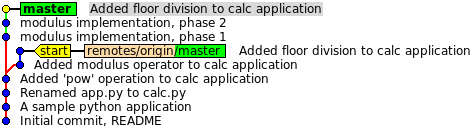
\includegraphics[width=0.75\linewidth]{gitrebase-split.png}
  \label{fig:gitrebase-split}
  \caption{Result of a split in a git rebase}
\end{figure*}

\noindent \textbf{Deleting and Reordering commits}

Finally, it's possible to delete and reorder commits.
To do so, simply delete and reorder lines in the interactive rebase editor.
This is left as exercice.

\bibliography{../common/refs}
\bibliographystyle{plainnat}

\end{document}


% \marginnote{}